% \pagebreak[4]
% \hspace*{1cm}
% \pagebreak[4]
% \hspace*{1cm}
% \pagebreak[4]

\chapter{Giới thiệu chung}
\ifpdf
    \graphicspath{{Chapter1/Chapter1Figs/PNG/}{Chapter1/Chapter1Figs/PDF/}{Chapter1/Chapter1Figs/}}
\else
    \graphicspath{{Chapter1/Chapter1Figs/EPS/}{Chapter1/Chapter1Figs/}}
\fi

\section{Phát biểu bài toán}
	Phân tích quan điểm là một trong những bài toán xử lý ngôn ngữ tự nhiên, đã và đang được nghiên cứu rộng rãi, cũng giống như bài toán phân loại văn bản, theo đó mỗi văn bản sẽ thuộc về một trong các lớp được xác định trước. Trong phân tích quan điểm, các câu đầu vào sẽ được phân loại vào các nhãn quan điểm phù hợp, cụ thể được chia thành hai loại như sau: \\
	\begin{itemize}[label = \textbullet]
		\item Binary class: Gồm 2 lớp quan điểm
		\begin{itemize}[label = \textendash]
			\item Tiêu cực(negative)
			\item Tích cực(positive)
		\end{itemize}
		\item Multi class: Gồm 5 lớp quan điểm
		\begin{itemize}[label = \textendash]
			\item Rất tiêu cực(very negative)
			\item Khá tiêu cực(somewhat negative)
			\item Không tích cực mà cũng không tiêu cực(neural)
			\item Khá tích cực(somewhat positive)
			\item Rất tích cực(very positive) \\
		\end{itemize}
	\end{itemize} 
Hiện nay, bài toán đang được áp dụng vào nhiều hệ thống khác nhau:
	\begin{itemize}[label = \textbullet]
		\item Hệ thống xếp hạng sản phẩm dựa trên các nhận xét, bình luận của khách hàng
		\item Hệ thống gợi ý
		\item Hệ thống lọc tin rác 
	\end{itemize}

\section{Deep Learning là gì?}
Deep learning là một kĩ thuật Machine Learning mạnh mẽ đang được nhiều người trong ngành biết đến và nghiên cứu. Kĩ thuật này nổi trội là do chúng thực hiện được hai việc cùng lúc: biểu diễn thông tin (represent problem/feature engineering) và học (learning). Do đó, kĩ thuật này còn được gọi là representation learning.

Bên cạnh các lĩnh vực đã gặt hái được nhiều thành công như Xử lý ảnh số và video số, hay Xử lý tiếng nói, Deep Learning cũng được áp dụng vào Xử lý ngôn ngữ tự nhiên. Với nền tảng là mạng nơ-ron(Neural Nerwork), Deep Learning hiện đang là một trong những kỹ thuật mạnh mẽ nhất và dữ liệu(Data) là một phần không thể thiếu trong kỹ thuật này. Dưới đây là kiến trúc cơ bản của mạng nơ-ron.\\
	\begin{center}
	  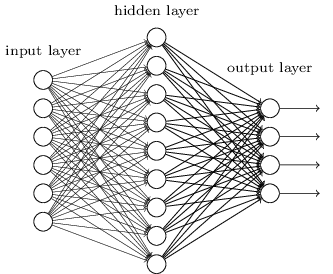
\includegraphics[width=0.55\textwidth]{neural}
	  \captionof{figure}{Kiên trúc Neral Network}  
	  \label{neural}
	\end{center}
Mạng nơ-ron cơ bản gồm 3 tầng chính:
	\begin{itemize}[label = \textbullet]
		\item Tầng đầu vào(input layer): Tẩng biểu diễn thông tin đầu vào, thường được biểu diễn bởi vector đặc trưng cho các thuộc tính của dữ liệu đầu vào
		\item Tầng ẩn: Biểu diễn, chắt lọc thông tin dữ liệu đầu vào qua các hàm kích hoạt(activation), được liên kết với tầng trước bởi ma trận trọng số.
		\item Tầng đầu ra(output layer): Biểu diễn thông tin đầu ra, kết quả mà chúng ta mong muốn.
	\end{itemize}
Các nhà khoa học là đã chứng minh rằng trên lý thuyết, với bộ dữ liệu đủ lớn thì chỉ cần một lớp ẩn duy nhất chúng ta có thể giải quyết được tất cả các bài toán. Nhưng trên thực tế để làm được điều này, số lượng nơ-ron ở tẩng ẩn sẽ rất lớn, có thể lên tới hàng tỉ nơ-ron và với tốc độ xử lý của các siêu máy tính hiện tại thì chúng ta không thể giải quyết vấn đề với chỉ duy nhất 1 tầng ẩn, thay vào đó mạng nơ-ron sẽ có thêm nhiều lớp ẩn hơn để phù hợp với từng bài toán.

 



